106. \begin{figure}[ht!]
\center{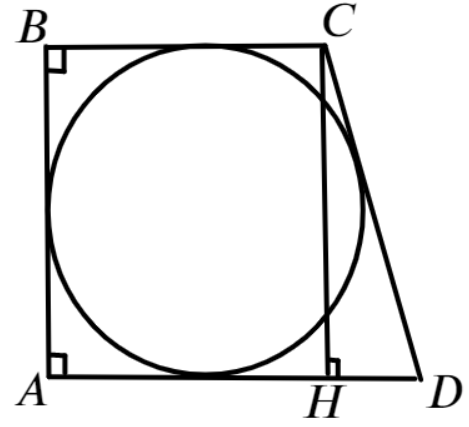
\includegraphics[scale=0.35]{g9-98.png}}
\end{figure}\\
Сторона $AB$ равна высоте трапеции и диаметру вписанной окружности, то есть $2R.$ Пусть $BC=x,\ HD=4R-x,$ тогда так как трапеция является описанной (суммы противоположных сторон равны), имеем $CD=4R+x-2R=2R+x.$ По теореме Пифагора для треугольника $CHD$ получаем $(4R-x)^2+4R^2=(x+2R)^2,\
x^2-8xR+16R^2+4R^2=x^2+4xR+4R^2,\ x=\cfrac{4}{3}R,\ CD=\cfrac{4}{3}R+2R=\cfrac{10}{3}R.$ Таким образом,
стороны трапеции равны $2R,\ \cfrac{4}{3}R,\ \cfrac{10}{3}R,\ 4R.$\\
